\openingarticle
\def\ppages{\pagerange{zidan:firstpage}{zidan:lastpage}}
\def\shorttitle{Treatment of Khedive Ismail’s antique gun (1863--1879)}
\def\maintitle{Treatment of Khedive Ismail’s antique gun (1863--1879) at the National Military Museum. A Case Study}
\def\shortauthor{Yassin E. Zidan, Nesrin M. N. El Hadidi, Maisa M.A. Mansour, Wael A.A. Abo Elgat}
\def\authormail{}
\def\affiliation{}
\def\thanknote{}
%--------------------------------------------------------------
\mychapter{Treatment of Khedive Ismail’s antique gun (1863--1879) \\ at the National Military Museum. A Case Study}
\begin{center}
	{\Large\scshape Yassin E. Zidan \footnote{Professor of Textile Conservation, Conservation Department, Faculty of Archaeology; Main fields of research are in Ancient Textile Technologies dating back to different periods of Egyptian history. The assessment of decay and deterioration of these objects and methods of their conservation and treatment are also part of his research. Additionally he supervises MA and PhD theses in the field of conservation of organic materials.}}\\  Cairo University\\[1em]
		
	
	{\Large\scshape 	Nesrin M. N. El Hadidi\footnote{Assistant Professor, Conservation Department, Faculty of Archaeology; Main fields of research are in Ancient Technologies of objects made of wood and plant related materials dating back to different periods of Egyptian history. The assessment of decay and deterioration of these objects and methods of their conservation and treatment are also part of her research, especially objects found or buried in dry environments.}}\\	
	\href{mailto:nelhadidi@gmail.com}{nelhadidi@gmail.com}\\
	 Cairo University \\[1em]
	
	
	{\Large\scshape 		Maisa M.A. Mansour\footnote{Assistant Professor, Conservation Department, Faculty of Archaeology; Main fields of research are in biodeterioration and biodegradation of old objects made of different materials whether organic or inorganic artifacts. Methods of conservation and treatment are also part of her research, Also has many published international researches in this field.}}\\ 
\href{mailto:maisamansour_40@yahoo.com}{maisamansour\_40@yahoo.com}\\
Cairo University \\[1em]


	{\Large\scshape 	Wael A.A. Abo Elgat\footnote{(\textit{Corresponding Author});  Assistant Lecturer; Main fields of research are in Ancient Technologies of objects made of wood in contact with metal especially iron dating back to different periods of Egyptian history. The assessment of decay and deterioration of these objects and methods of their conservation and treatment are also part of his research. He also has many published international researches in this field.}}\\
\href{mailto:watsat20@yahoo.com}{watsat20@yahoo.com}\\
High Institute of Tourism, Hotel Management and Restoration\\ Alexandria, Egypt

\end{center}
\vspace{3em}
\midarticle
%--------------------------------------------------------------
\label{zidan:firstpage}
%\newcommand\authorname{Replace-me-with-the-author’s-name}

%----------------------------------------------------------------------------------------
	\begin{myabstract}
 In this\marginnote{Abstract} case study Khedive Ismail’s antique gun, which is currently kept at the National Military Museum in Cairo, is documented and treated. The antique gun with a handgrip was made up of a spear of wood, a barrel and a blow up instrument made from iron.  The maximum handgrip width of the gun is about \SI{9.4}{\centi\meter} and its total length with wood spear is \SI{113}{\centi\metre}. The gun deteriorated throughout the years due to neglect and inappropriate exhibition conditions at the museum which included; relative humidity, temperature, and the accumulation of air dust particles and aerosols inside the inadequately sealed display cases. This resulted in the manifestation of heavy metal rust in the pipe, especially underneath the wooden spear, in addition to the formation of dust and rust stains on the wood.

This research explains the treatment and restoration steps of the archaeological gun and illustrates the actual scientific procedures that were followed, starting from the documentation, followed by the analysis and scientific tests which were carried out to identify the components and archaeological parts of the gun, concluded by the actual stages of restoration and conservation.
		
\keywords[Keywords]{Wood, Iron, Rust, Gun, Conservation, Treatment, Analysis.}
	\end{myabstract}

%\section{Introduction}
	
\lettrine[nindent=0em,lines=3]{T}{his} paper deals with an applied study on an antique gun, which is in the collection of the National Military Museum at Saladin Citadel in Egypt, the standing evidence for the victories of the Egyptian army and the heroism of the Egyptian soldier; who was described by Napoleon as the finest soldiers in the world. The Museum illustrates the story of the Egyptian military forces since ancient times until our modern age, illustrating a large number of battles and wars where the Egyptian army showed great skills \parencite{Seaman_2013}.
	
	This gun belongs to Ismail Pasha, who was the Khedive of Egypt and Sudan during the XIX century (1863 to 1879). Ismail's khedivate is closely connected to the construction of the Suez Canal \parencite[49--55]{Dye_1880}. 
	
	In previous research the preservation of a rare French pistol of the Revolutionary period which had been found after resting for 185 years on the wreck of \textit{Le Cygne} (1808) was described. Treatment and restoration stages included general description, magnetic examination and interpretation, X-ray examination, cleaning of the cavities and treatment of different materials, such as wood and the brass mounting \parencite[161-169]{Mardikian_1996}. 
	
	In a study the effect of iron rust on wood in an archaeological gun (No. 7 / 14 at the Museum of Applied Arts, Helwan University) was documented and the procedures for the treatment and restoration of the gun were explained \parencites[285--290]{AboElgat_2010}[348--353]{Zidan_2011}.
	
	In another study the treatment and restoration methods of an antique sword dating back to the Ottoman period (\nth{13} AH/\nth{19} \AD century) at the National Military Museum-Saladin Citadel in Egypt, are clearly explained, including the actual scientific procedures that had been followed during the restoration and treatment, starting from the archaeological documentation, the analysis and scientific tests which were carried out to identify the components and archaeological parts of the sword, and the actual stages of restoration and conservation \parencite[1-6]{Zidan_2013}.
	
	In this research the effect resulting from the precipitation and interpenetration of rust from the iron metal into the wood fibers is studied. The physiomechanical and chemical properties of wood which are correlated with these metals were the main points, in addition to the deformation that takes place in the appearance of wood as a result of its spotting or blotting with the residue of the rust on the surface of wood.  
	
The identification of damage, which occurs on wood as a result of these factors helped study the possibility of how to minimize the dual effect of wood and metals on each other in archaeological materials. Treatment and repair included several stages, but prior to these stages a study and detailed documentation of the guns’ condition was completed. 

The dimensions were measured carefully and photographed, the gun was closely examined and samples were analyzed to identify the components of the metal parts. The condition and degree of damage was evaluated, and the materials used in previous restoration were documented. Then the practical procedures for repairing and maintaining the gun, which involved disassembly and cleaning of all of its components, strengthening, blocking and filling gaps and cracks, followed by isolating, reassembling and putting the pieces together correctly once again.

%\section{Materials and Methods}

%\subsection{Analysis}

Analysis\marginnote{Materials and Methods -- Analysis}  and investigation were undergone using infra-red spectroscopy (FTIR \SIrange{400}{4000}{\centi\metre}\textsuperscript{-1} +ATR unit), Atomic absorption analysis (analytic Jena instruments- Conter. AA 700), X-ray diffraction (Philips, Diffractometer type: PW1840, Generator tension: 40KV, Wavelength Alpha1: 1.54056A°, Start angle: 4.025, End angle: 69.975, Maximum intensity: 67.24), light microscope and Scanning Electron Microscope with E.D.X (operator: EM unit Fac. Sc.; All ISIS users: Demonstration Data SiLi detector and LV5400 model 2005).

%\subsection{Treatment}

For \marginnote{Treatment} treatment and restoration of the gun the following procedures were applied:

\begin{enumerate}
	\item Dust and damage in the form of cracks and separations internally and externally and old varnish layers from the different parts of the gun (Fig. \ref{fig:Fig1}a-d and \ref{fig:Fig2}a) were cleaned using mechanical techniques, such as different types of brushes and scalpels \parencite[143]{Unger_2001}, which were suitable for both wood and metal.
	\item The state of the gun allowed easy handling, and the metal parts that had been attached to previously added wood in old restoration (Fig. \ref{fig:Fig2}a, b, d) were separated from the gun.  \parencites[1--2]{Davis_1998}[1--15]{Zelinka_2005}.
	\item Chemical cleaning and the removal of the remains of materials used in earlier treatment, e.g. the old varnish (as identified by FTIR) which heavily covered both the metal and wooden parts of the gun, was removed from the metal parts using acetone and from the wooden parts using 95\% ethyl alcohol (from: El-Nasr Company for Intermediate Chemicals). Distilled water and ethyl alcohol 95\% with different mixture ratios 1:1, 2:1, respectively was applied to clean surface dirt, Ammonia solution (2\%) was used to clean the dark strong dirt from the outside of the wooden handle of the gun (Fig. \ref{fig:Fig2}c). 
	\item Cleaning of the remains of iron rust formed under the barrel, was applied by using a diluted solution of oxalic acid 1-2\% in hot distilled water \parencites[5]{William_1999}[1--20]{Williams_2002} followed by washing off the previously cleaned parts with acid using distilled water several times.
	\item The separate parts and crack in the longitudinal wooden part were reassembled together using Paraloid B72. The upper parts of the wooden handle, as well as the area below the screws, were completed in order to reinstall the lock plate correctly using balsa wood (\textit{Ochroma pyramidale}) \parencite[4--11]{Newman_2013}. The lacunae around the completion parts were filled with a mixture of glass microballoon and soft wood sawdust with Paraloid B72 (5\% w/v) dissolved in ethanol + acetone (40:60) (Fig. \ref{fig:Fig3}c).
	\item The metal parts that had been disassembled and removed from the gun were cleaned using a solution of citric acid 3-5\% by soaking and mechanical cleaning. This process was repeated several times until rust was removed. Rochelle salt solution was used for cleaning copper parts, followed by washing all the parts with distilled water using hot-cold cycles several times to prevent the future effects of solutions on the metal or to maintain the pH value. Finally, the parts were dried with 95\% ethyl alcohol (Fig. \ref{fig:Fig3}a,b).
	\item Heavy black rust, in certain parts of the barrel was cleaned chemically by soaking using EDTA solution (Ethylene Diamin Tetracetate - Komplexon3 %make this a small three
	) with a pH reaches to 5.5 by adding concentrated acetic acid \parencite[225]{Sobhy_2006}. To increase the effect of the cleaning process and to remove a layer of iron oxide magnetic black (magnetite), which has a scarce solubility, the powder of Komplexon3 was added on the black portions locally. After every application, the powder was mechanically cleaned to remove the dissolved corrosion products, until the desired effect of cleaning was reached, commensurate with the case taking into account the preservation of the patina layer. This was then followed by washing with distilled water, hot then cold, and drying with ethyl alcohol. This was followed by isolation of all parts of the gun immediately after drying using two cross layers of Paraloid B72 dissolved in toluene 4\% (Fig. \ref{fig:Fig3}d).
	\item 25 shot cartridges of iron, lead alloy (identified by Atomic absorption) were wrapped with a piece of tissue paper in the presence of the remains of gunpowder which was discovered while cleaning the inside of the iron barrel (Fig. \ref{fig:Fig3}b).
	\item In the last step all the parts were reinstalled using the screws that also had been previously cleaned and isolated. Then parts of the iron rings were put in place along the iron barrel to link between them and the parts of wood underneath (Fig. \ref{fig:Fig10}).
\end{enumerate}

\begin{figure}[!htb]
	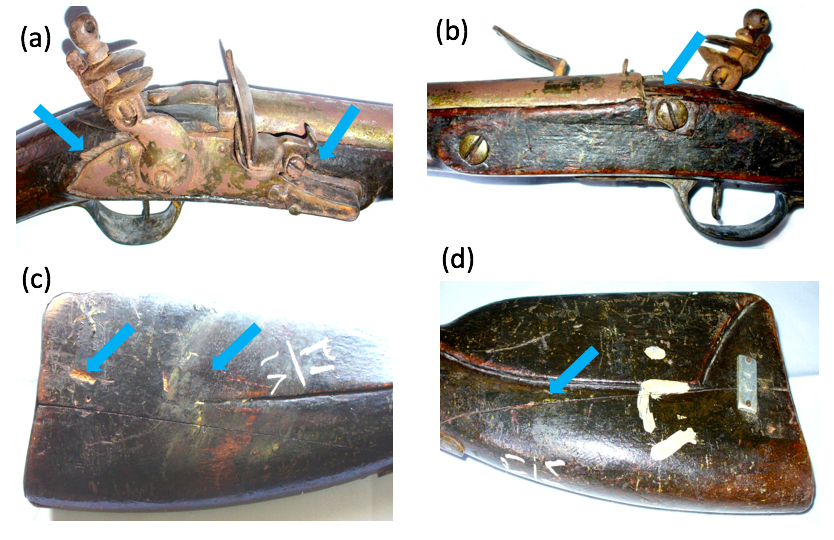
\includegraphics[width=\linewidth]{figures/zidan_Fig1}
	\caption{Shows the gun before treatment; a,b- lock plate of the gun showing iron rust and the heavy bright layers of varnish covering the hall handle, c,d- show damage in the form of cracks and separations in the wooden handle of the gun and deformation, heavy dust, black layers, human deterioration on the wooden stock of the handle. Figure by Wael A.A. Abo Elgat.}
	\label{fig:Fig1}
\end{figure}
\begin{figure}[!htb]
	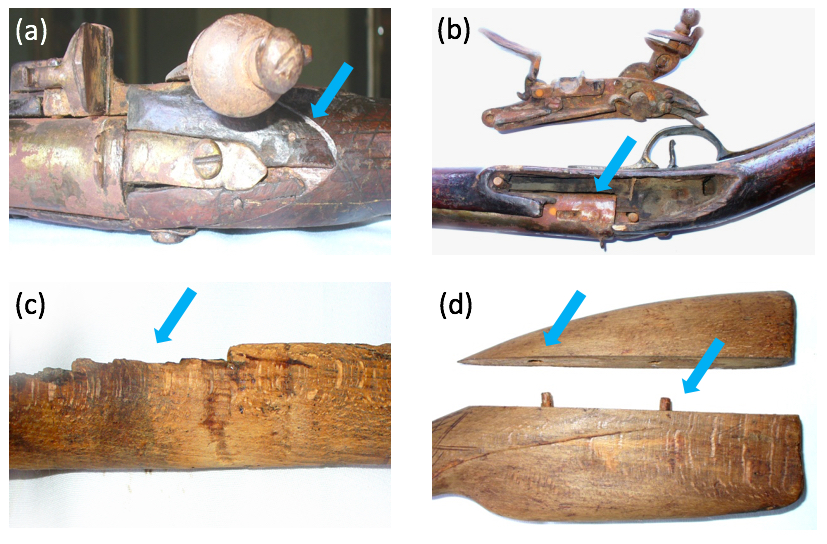
\includegraphics[width=\linewidth]{figures/zidan_Fig2}
	\caption{Shows the gun during and after treatment; a- the deformation and separated wood above the handle. b- during investigation and cleaning of the wood underneath lock plate. c- stages of localized initial chemical cleaning of soot in wooden surface, d- the stock after cleaning during assembling two parts. Figure by Wael A.A. Abo Elgat.}
	\label{fig:Fig2}
\end{figure}
\begin{figure}[!htb]
	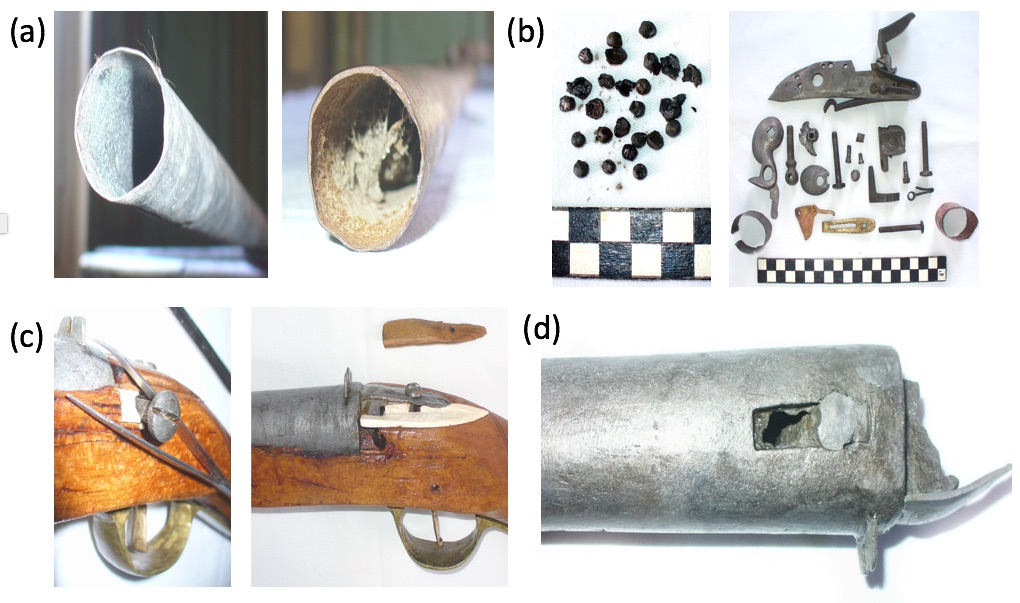
\includegraphics[width=\linewidth]{figures/zidan_Fig3}
	\caption{Shows the gun during and after treatment; a- part of the barrel before and after cleaning, b- the different metal parts of the lock plate and the shot cartriges during cleaning, c- the use of balsa in reconstruction and repair, d- part of the barrel after cleaning. Figure by Wael A.A. Abo Elgat.}
	\label{fig:Fig3}
\end{figure}
%\section{Results}
After\marginnote{Results} examination and analysis of the different parts of the gun, documentation of technique and materials used to make the gun was possible. The state of preservation was recorded prior to the repair and conservation stages. The following results were obtained: 

\begin{enumerate}
	\item By comparing the results obtained from analyzing the remains of an old lacquer used on most parts of the gun with several natural lacquers using FTIR it turned out that dammar resin was used as a coating (Fig. \ref{fig:Fig4}). 
	\item Samples taken from rust products from different parts of the gun were analyzed using X-ray diffraction. The bottom of the barrel and inside the nail holes were affected by iron rust from surrounding metal parts and the impact of air pollution in the atmosphere of the museum had increased the damage (Fig. \ref{fig:Fig6}, \ref{fig:Fig7}).  
	\item Examination of the sample from the wooden handle (the stock) of the gun using optical microscope proved that it was made of beech wood \textit{Fagus sylvatica L.}, according to literature. Pore Distribution: Diffuse-porous; growth rings distinct, Pores: Small, solitary and in irregular multiples and clusters, numerous and evenly distributed throughout most of the ring; narrow but distinct latewood in each ring due to fewer, smaller pores, Rays: Largest rays conspicuous on all surfaces; darker ray fleck against lighter background on radial surfaces \parencite[117--118]{Hoadley_1990}(Fig. \ref{fig:Fig8}a,b).
	\item Analysis of the sample from the remains of the gunpowder with X-ray diffraction, X-ray fluorescence unit attached to scanning electron microscope (EDX), and FTIR + ATR confirmed that the gunpowder consists of saltpeter (potassium, or sodium nitrate), sulphur and charcoal (carbon) \parencites[3]{Driel_2000}[3--5]{Alexander_2012}[5]{Richard_2011} (Fig. \ref{fig:Fig5},\ref{fig:Fig7},\ref{fig:Fig9}).
	\item  For confirmation of the elemental composition of the rusted products from the barrel and lock plate, small samples from the rusted products were analyzed by an X-ray fluorescence unit attached to scanning electron microscope (EDX). The main component of the metals was made up of iron, where it appeared in high rates, mixed with a very small percentage of elemental traces of iron rust component.
	\item Analysis of metal parts from the gun by Atomic Absorption-Flame technique, showed that the first piece of metal that was connected to the wooden part with iron barrel, the lock plate and barrel were made of iron, whereas the shot cartridges were made of iron- lead alloy (50\% iron, 50\% lead). 
\end{enumerate}

\begin{figure}[!htb] 
	\begin{minipage}[b]{0.5\linewidth}
		\centering
	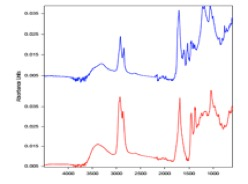
\includegraphics[width=.9\linewidth]{figures/zidan_Fig4}
	\caption{Shows FTIR+ATR spectra of sample analysis of the old lacquer taken from the barrel surface of the gun (top), that similar to the dammar resin - control (bottom).}
	\label{fig:Fig4}
	\end{minipage} 
	\begin{minipage}[b]{0.5\linewidth}
		\centering
		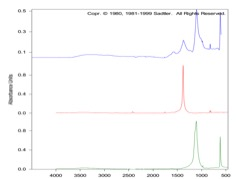
\includegraphics[width=.9\linewidth]{figures/zidan_Fig5}
		\caption{Spectra of sample analysis of the gunpowder (top) by FTIR+ATR are similar to the sample spectrum of potassium nitrate (middle), and potassium sulfate (bottom).}
		\label{fig:Fig5}
	\end{minipage} 
\end{figure}


\begin{figure}[!htb]
	\begin{minipage}[b]{0.5\linewidth}
		\centering
		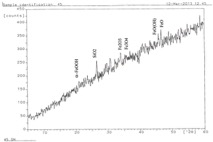
\includegraphics[width=.9\linewidth]{figures/zidan_Fig6}
		\caption{X-ray diffraction pattern of the sample taken during the cleaning of the entire parts of the lock plate, showing iron rust components.}
		\label{fig:Fig6}
	\end{minipage} 
	\begin{minipage}[b]{0.5\linewidth}
		\centering
		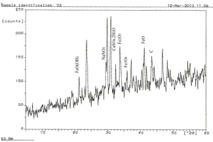
\includegraphics[width=.9\linewidth]{figures/zidan_Fig7}
		\caption{X-ray diffraction pattern of a sample of the gunpowder from the barrel showing that it contains iron rust compounds, carbon, sulfur and nitrate.}
		\label{fig:Fig7}
	\end{minipage} 
\end{figure}

\begin{figure}[!htb]
	\begin{minipage}[b]{0.55\linewidth}
		\centering
		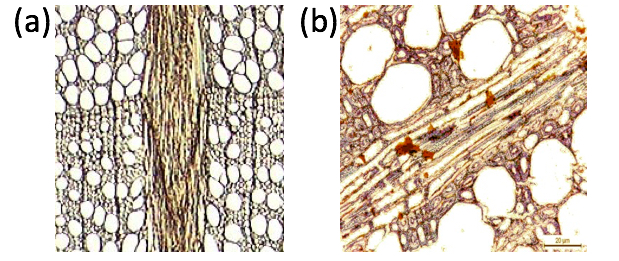
\includegraphics[width=.9\linewidth]{figures/zidan_Fig8}
		\caption{Cross sections of Beech wood (\textit{Fagus sylvatica L.}) on light microscope (a) standard from \textcite{Richter_2000}, (b) sample taken from the handle of the gun (20µm).}
		\label{fig:Fig8}
	\end{minipage} 
	\begin{minipage}[b]{0.45\linewidth}
		\centering
		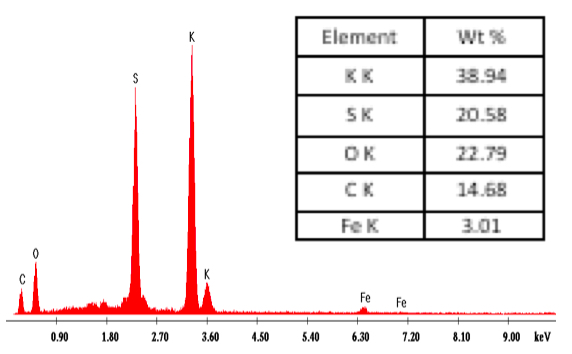
\includegraphics[width=.95\linewidth]{figures/zidan_Fig9}
		\caption{Results of elemental analysis EDX of a sample of gunpowder from the inside the barrel of the gun, showing the chemical components of the old gunpowder (saltpetre (potassium), sulphur and charcoal (carbon).}
		\label{fig:Fig9}
	\end{minipage} 
\end{figure}

\begin{figure}[!htb]
	\centering
	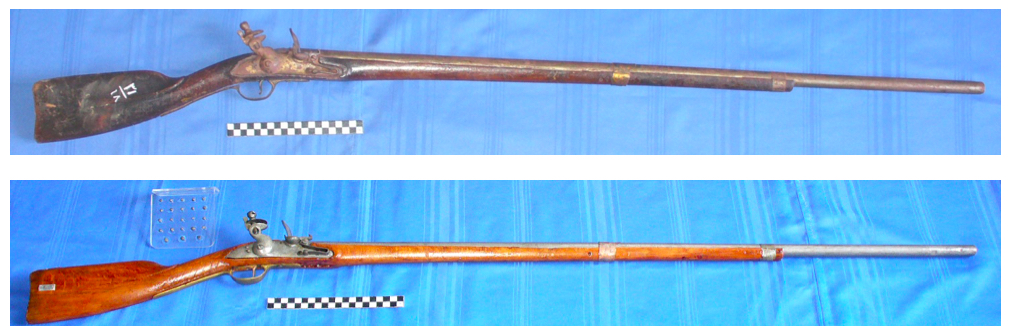
\includegraphics[height=.55\linewidth,angle=90]{figures/zidan_Fig10}
	\caption{The gun before (top), after cleaning and isolation (bottom).}
	\label{fig:Fig10}
\end{figure}
%\section{Conclusion}
X-ray\marginnote{Conclusion} diffraction, light microscope and Scanning Electron Microscope with E.D.X, Atomic Absorption analysis and Infra-Red spectroscopy techniques are important tools that help archaeologists and conservators to understand the nature and state of preservation of a complex composite object like the gun mentioned in this case study. Additionally the examination and analysis of the gun have helped explain the methods used in manufacture and reconstruction of guns dating back to this period. 

The authors explain the treatment and restoration steps of this gun and illustrate the actual stages that were carried out. 
\myseparator
%\section{Acknowledgements}
The\marginnote{Acknowledgements} authors would like to express special thanks to the ministry of Defense and the National Military Museum-Saladin Citadel in Egypt Administration for their support. 


\printbibliography[heading=subbibnumbered] 
\label{zidan:lastpage}
\closingarticle
